
\def\dX{6.0}
\def\dY{3.0}
\def\dR{0.7}

  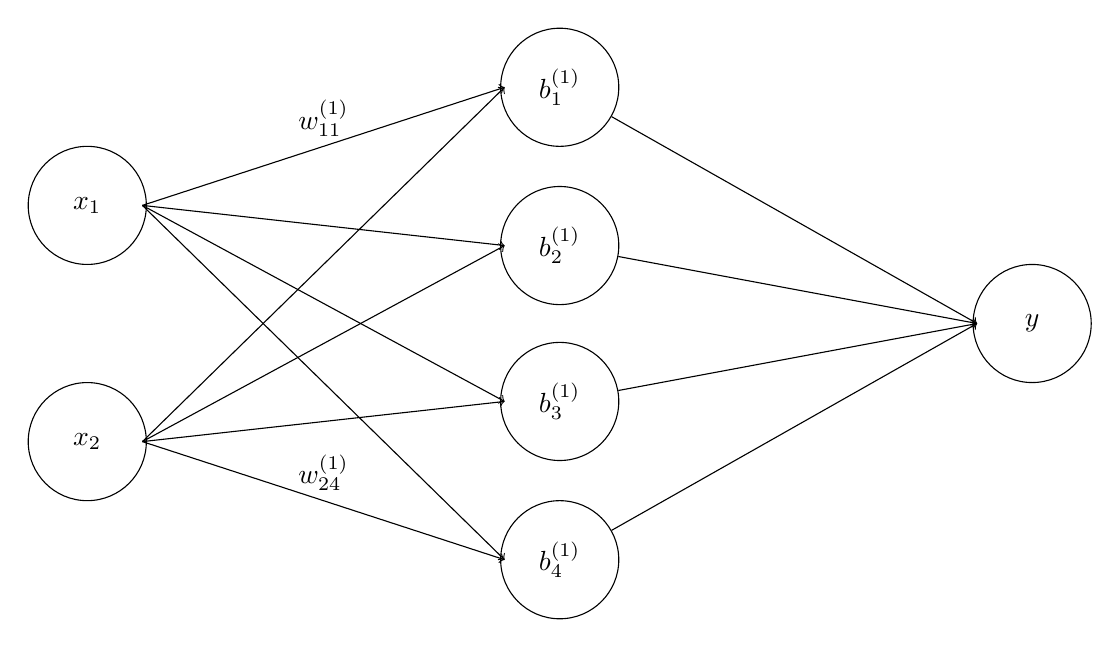
\begin{tikzpicture}
    %%   (lable)  (x, y)     {\text}
    \coordinate (CX1) at (-\dX+\dR,  0.50*\dY);
    \coordinate (CX2) at (-\dX+\dR, -0.50*\dY);

    \coordinate (CN1) at (    -\dR,       \dY);
    \coordinate (CN2) at (    -\dR,  0.33*\dY);
    \coordinate (CN3) at (    -\dR, -0.33*\dY);
    \coordinate (CN4) at (    -\dR,      -\dY);

    \coordinate (CY)  at ( \dX-\dR,         0);

    \node[shape=circle,draw=black, minimum size=1.5cm] (X1) at (-\dX,  0.50*\dY) {$x_1$};
    \node[shape=circle,draw=black, minimum size=1.5cm] (X2) at (-\dX, -0.50*\dY) {$x_2$};


    \node[shape=circle,draw=black, minimum size=1.5cm] (N1) at (0,      \dY) {$b_1^{(1)}$};
    \node[shape=circle,draw=black, minimum size=1.5cm] (N2) at (0, 0.33*\dY) {$b_2^{(1)}$};
    \node[shape=circle,draw=black, minimum size=1.5cm] (N3) at (0,-0.33*\dY) {$b_3^{(1)}$};
    \node[shape=circle,draw=black, minimum size=1.5cm] (N4) at (0,     -\dY) {$b_4^{(1)}$};

    \node[shape=circle,draw=black, minimum size=1.5cm] (Y)  at (+\dX,         0) {$y$};

    \path[->] (CX1) edge node[above] {$w_{11}^{(1)}$} (CN1);
    \path[->] (CX1) edge                              (CN2);
    \path[->] (CX1) edge                              (CN3);
    \path[->] (CX1) edge                              (CN4);

    \path[->] (CX2) edge                              (CN1);
    \path[->] (CX2) edge                              (CN2);
    \path[->] (CX2) edge                              (CN3);
    \path[->] (CX2) edge node[above] {$w_{24}^{(1)}$} (CN4);

    \path[->] (N1) edge (CY);
    \path[->] (N2) edge (CY);
    \path[->] (N3) edge (CY);
    \path[->] (N4) edge (CY);

  \end{tikzpicture}
